This sections includes further details on the interfaces between the custom internal components of the system and the IBM micro-services illustrated before. The communications among components should take place only through APIs, some of them need to be custom developed and others are already exposed by the services described in \ref{microservices}.
\\ A list of APIs needed for the application's well being are briefly described in the following list, grouped by functionality that interacts through them:

\textbf{User Data Management:}
\begin{itemize}
	\item \textbf{[POST] changePassword(userId,newPassoword):} Used from the client application to change the password of its user.
	\item \textbf{[POST] banUser(userId):} Used from the officers portal in order to ban a malicious user of the application.
\end{itemize}
the \textit{login} and \textit{register} interfaces are not described here since they are provided by the IBM App ID service.

\textbf{Violations:}
\begin{itemize}
	\item \textbf{[POST] createViolation(vData, URLs):} Used from the client application when a user wants to send a new ticket violation. The URLs of the picture are attached and point to objects in the Object Storage System.
	\item \textbf{[POST] sendAutomaticTicket(data, URLs):} Used when the user wants to send an automatic ticket. The URLs of the picture are attached and point to objects in the Object Storage System.
	\item \textbf{[GET] getViolationById(violationId):} Used from the officers portal to get the information of a specific violation.
	\item \textbf{[GET] getViolationsByUser(userId):} Used from the client application to get all the user's violations.
	\item \textbf{[GET]	getPendingTickets():} Used from the officers portal to get all the tickets that are yet to be processed.
	\item \textbf{[GET]	getPendingViolations():} Used from the officers portal to get all the violations that are yet to be processed.
	\item \textbf{[POST] approve(ticket):} Used from the officers portal to approve a ticket that was initially marked as invalid from the Tickets Check service.
	\item \textbf{[POST] changeViolationState(violationId,newState):} Used from the officers portal to change the status of a violation just analyzed from PENDING to ACCEPTED/DENIED.
	\item \textbf{[GET] getPositionWithGPS(x-coordinates,y-coordinates):} Used from the client application to get the user's position given their GPS position.
\end{itemize}

\textbf{Data Mining:}
\begin{itemize}
	\item \textbf{[GET] getLicensePlate(images,oldLicensePlates):} Used from the client application to get a license plate from the images provided if found. The API should also accept a set of wrong license plate in case the precedent output of the API call was wrong and the user realized that the license plate given didn't correspond to the actual license plate of the vehicle committing the violation.
	\item \textbf{[POST] checkTicket(data):} Used by the Tickets checking service to check if the ticket might no be legit.
	\item \textbf{[GET] querySuggestions():} Used by the Suggestions service to query for new suggestions.
	\item \textbf{[POST] sendViolation(vData, metadata):} Used by the Violations service to send new violations into the data mining engine
\end{itemize}

\textbf{Tickets Check:}
\begin{itemize}
	\item \textbf{[POST] sendTicket(data):} Called when the violation service receives an automatic ticket, is used to check if the ticket might not be legit.
\end{itemize}

\textbf{Tickets Hashing System:}
\begin{itemize}
	\item \textbf{[POST] sendTicket(data):} Called when the violation service receives an automatic ticket, is used to store the hash into the microservice.
	\item \textbf{[GET] checkHash(hash):}  Used from the officers portal to check the integrity of a specific violation (chain of trust). 
\end{itemize}

\textbf{Statistics:}
\begin{itemize}
	\item \textbf{[GET] getAreaInformation(area):} Used from both the client application and the officers portal to retrieve the information of an area that may be unsafe (both) or not (only officers).
	\item \textbf{[GET] getWorstDriversInformation():} Used from both the client application and the officers portal to retrieve the information about the worst drivers in the SafeStreets database. The officers should be able to acknowledge more information of the drivers than the users.
	\item \textbf{[GET] getData(bounds):} Used from both the client application and the officers portal to get the information of a specific thing given some proper bounds.
	\item \textbf{[GET] getStatisticsOverview:} Used from the client application so that the user could have a more general idea when he accesses the statistic section.
	\item \textbf{[POST] sendViolation(vData, metadata):} Used by the Violations service to send new violations into the statistics database
\end{itemize}

\textbf{Suggestions:}
\begin{itemize}
	\item \textbf{[GET] getSuggestions():} Used by the officers to get new suggestions.
	\item \textbf{[POST] delete(suggestion):} Used by the officers to delete a managed suggestion.
\end{itemize}

Of course, the mentioned above APIs are not to be intended as strict and not-modifiable, but there can be added, removed or edited APIs to/from the list during the implementation of the application if there is the need to use a different approach.

In order to provide the correct application functioning, it is trivial to say that all the components needs to expose APIs that can allow them to be in communication with each others.

\begin{center}
	\begin{figure}[htp] 
		\makebox[\textwidth][c]{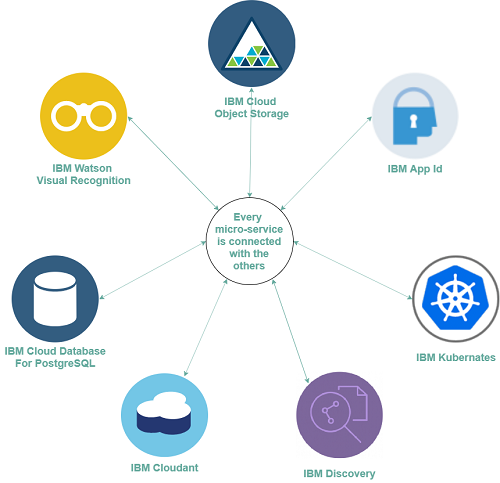
\includegraphics[width=0.87\textwidth]{images/components}}
		\label{fig:components} 
	\end{figure} 
\end{center}
